% ****** Start of file apssamp.tex ******
%
%   This file is part of the APS files in the REVTeX 4.2 distribution.
%   Version 4.2a of REVTeX, December 2014
%
%   Copyright (c) 2014 The American Physical Society.
%
%   See the REVTeX 4 README file for restrictions and more information.
%
% TeX'ing this file requires that you have AMS-LaTeX 2.0 installed
% as well as the rest of the prerequisites for REVTeX 4.2
%
% See the REVTeX 4 README file
% It also requires running BibTeX. The commands are as follows:
%
%  1)  latex apssamp.tex
%  2)  bibtex apssamp
%  3)  latex apssamp.tex
%  4)  latex apssamp.tex
%
\documentclass[%
 reprint,
%superscriptaddress,
%groupedaddress,
%unsortedaddress,
%runinaddress,
%frontmatterverbose, 
%preprint,
%preprintnumbers,
%nofootinbib,
%nobibnotes,
%bibnotes,
 amsmath,amssymb,
 aps,
%pra,
%prb,
%rmp,
%prstab,
%prstper,
%floatfix,
]{revtex4-2}

\usepackage{graphicx}% Include figure files
\usepackage{dcolumn}% Align table columns on decimal point
\usepackage{bm}% bold math
\usepackage{physics}
\usepackage{mathtools}
\usepackage{hyperref}
\hypersetup{hidelinks}
%\usepackage{hyperref}% add hypertext capabilities
%\usepackage[mathlines]{lineno}% Enable numbering of text and display math
%\linenumbers\relax % Commence numbering lines

%\usepackage[showframe,%Uncomment any one of the following lines to test 
%%scale=0.7, marginratio={1:1, 2:3}, ignoreall,% default settings
%%text={7in,10in},centering,
%%margin=1.5in,
%%total={6.5in,8.75in}, top=1.2in, left=0.9in, includefoot,
%%height=10in,a5paper,hmargin={3cm,0.8in},
%]{geometry}
\usepackage{booktabs}
\begin{document}

\preprint{APS/123-QED}

\title{Nonlinear Effects in Fiber-optical Communication}% Force line breaks with \\

\author{Wentao Li}
 \affiliation{Physics Department, 
                Fudan University\\
            Department of Physics, 
            University of California Berkeley}%Lines break automatically or can be forced with \\


\date{\today}% It is always \today, today,
             %  but any date may be explicitly specified

\begin{abstract}
    An overview of fiber-optical communication 
    is given, with an emphasize on nonlinear aspects 
    of fiber optics. 
    Various phase modulation effects, 
    four wave mixing and 
    solitons are discussed. 
    Such nonlinear effects 
    turn out to host potentials of 
    improving performance in 
    communication systems. 
    Based on the current challenges of 
    fiber-optic communication, methods for 
    improving fiber-optic communication systems 
    that exploit nonlinear properties are proposed. 
\end{abstract}

%\keywords{Suggested keywords}%Use showkeys class option if keyword
                              %display desired
\maketitle

%\tableofcontents
\section{Introduction}
As the backbone of modern communication infrastructure, 
fiber-optic systems are crucial for 
the transmission of information. 
\par
Because of the small cross section of fiber core 
and the long distance over which optical signals travel, 
nonlinear effects in fibers are strong.
\cite{agrawal_fiber-optic_2022} 
They can either disrupt or improve the performance 
of fiber-optic transmission systems. 
Turning disruption into imrpovement requires 
physical insight as well as engineering ingenuity. 
\par
The past few decades have seen remarkable 
achievements in fiber-optic communication 
that are aided by a better understanding of 
nonlinear properties of optical fiber, including 
ultra-long haul transmission with solitons, 
dispersion management via optical phase conjugation, 
dense wavelength-division multiplexing and 
space-division multiplexing through multicore fibers. 
\par
It is therefore necessary to understand and 
take advantage of nonlinear phenomena in fibers 
so that challenges are better understood and 
solutions become more robust. 
\par
In this paper, a historical account as well as 
basic concepts of fiber-optic communication 
will be given to facilitate an understanding 
of past achievements, typical techniques and open problems. 
Based on that, 
current challenges and techniques involving nonlinear phenomena 
will be discussed in more detail. 
Finally, proposals of utilizing nonlinear effects 
for fiber-optic communication will be made. 
We will also comment on the relation between 
the physics of nonlinear optics 
and the engineering aspects of fiber communication.
\par
We do not attempt at a comprehensive 
analysis of fiber-optic communication \textit{systems}, 
which comprise of not only fibers, but also 
encoders (also known as modulators), decoders and amplifiers. 
Instead, focus on fibers is kept throughout the paper 
in order for the physical perspective to 
emerge from various engineering technicalities. 
Neither will we discuss \textit{digital} techniques 
in too much depth, because they are 
primarily implemented in the encoders and decoders 
instead of fibers. 
\section{History and Overview}
In this section we provide an overview of 
fiber-optic communication technogies. 
We start with basic concepts of communication 
and optic fiber to introduce core ideas as well as 
technical terms. 
More physical detail, especially those related to 
nonlinear effects, will be given in later sections. 
\subsection{Basic Concepts of Communication}
In fiber-optic communication, 
a \textbf{signal} is a function of time that 
encodes information. 
If the function can take continuous values, 
then it corresponds to 
an \textbf{analog signal}; otherwise 
it corresponds to a \textbf{digial signal}. 
Any analog signal can be \textbf{quantized} 
into a digital signal with a certain amout of 
noise that is inherent to the quantization process. 
\begin{figure}[h]
    \centering
    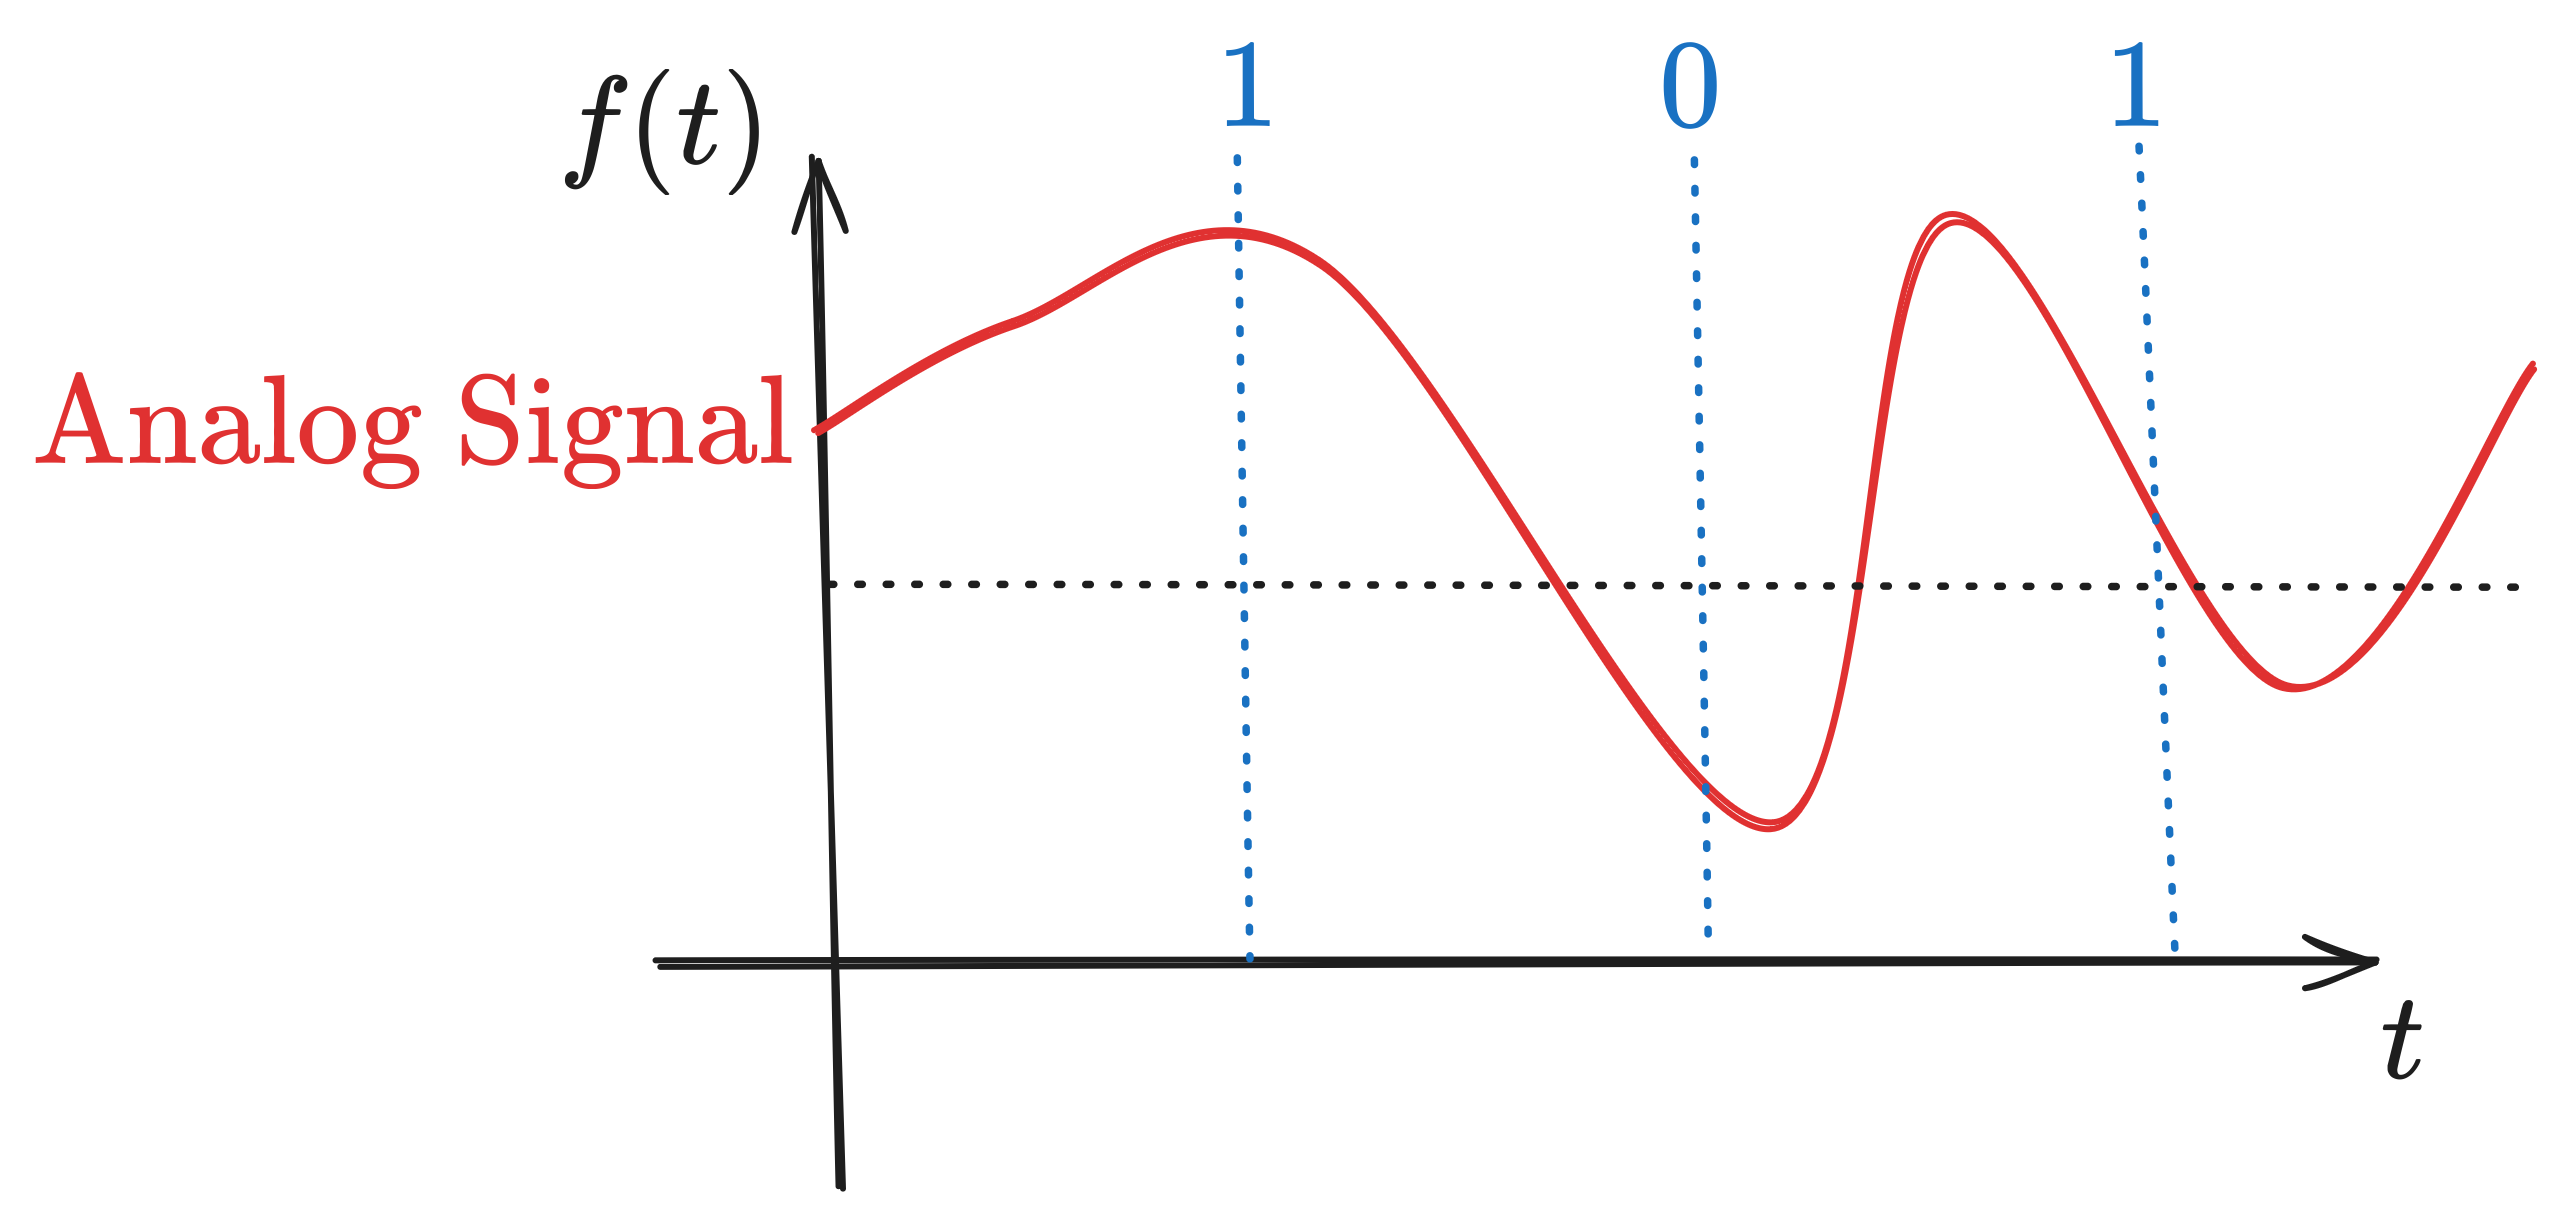
\includegraphics[width=0.4\textwidth]
    {images/AnalogVSDigital.png}
    \caption{Example of analog and digital signal. 
    Red line is an analog signal; 
    blue binary numbers are the 
    digital signal bits after quantization. 
    In this figure, the rightmost bit 1 
    contains more quantization noise than the rest two bits.}
\end{figure}
\par
Because of the digital nature of most data that 
needs transmission, fiber-optical systems transmit 
digital signals. 
The \textbf{bit slot} $T_{B}$ is the time duration which 
one bit of information occupies in the signal. 
The \textbf{bit rate} $B$ is the rate at which 
bits are transmitted, therefore $B=1 /T_{B}$. 
A simple modulation format is to use 
a non-empty bit slot for encoding ``1'' and 
an empty one for ``0''. This is the 
\textbf{binary signal}. 
A typical quantity depicting the capability of 
communication systems is $BL$, the product of bit rate 
and the distance of transmission. 
\par
A \textbf{channel} is a collection of signals 
that are transmitted within the same physical system. 
In order for different signals to not disrupt each other, 
signals should either be delayed in time or 
occupy different frequencies. 
\par
Multiple channels can be transmitted 
within the same physical system. 
This is known as channel \textbf{multiplexing}, which is 
essentially parallel transmission of channels 
\textit{without} additional physical cost. 
\par
For example, if the bit slot is longer than the pulse of one bit, 
then the surplus amount of time can be exploited to achieve 
channel multiplexing. 
This is known as 
\textbf{time-division multiplexing} (TDM). 
Similarly, if the physically allowed bandwidth 
is larger than the single-channel bandwidth, 
then the surplus of bandwidth can be exploited to 
carry multiple channels. 
This is known as \textbf{wavelength-division multiplexing} (WDM).
\begin{figure}[h]
    \centering
    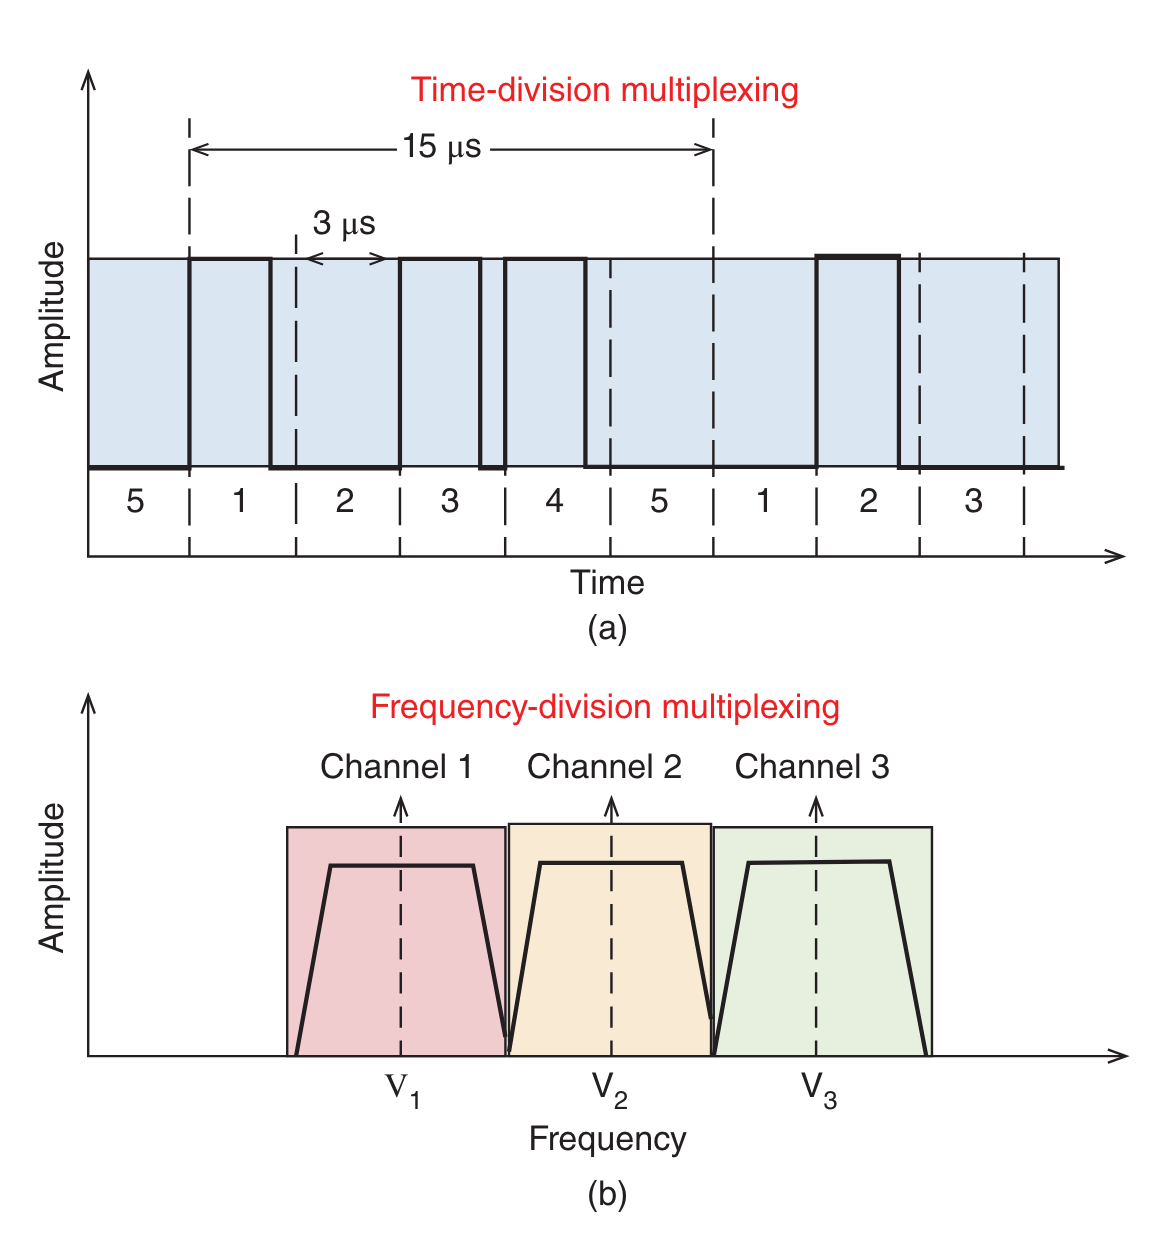
\includegraphics[width=0.4\textwidth]{images/ChannelMultiplexing.png}
    \caption{Diagram for TDM and WDM. 
    In the figure the term 
    ``frequency division multiplexing'' 
    is used intead of WDM. 
    Reproduced from \cite{agrawal_fiber-optic_2022}.}
\end{figure}
\par
Other multiplexing techniques include 
\textbf{Space-division Multiplexing} (SDM) and 
\textbf{Coherent Detection}, which is 
to encode information not only in the amplitude 
but also in the phase of optical signals. 
\par
Multiplexing techniques can be 
assembled in a hierarchical manner. 
For example, in WDM each frequency may contain 
several channels that are separated via TDM or 
other multiplexing techniques. 
This fact opens up rich opportunities for multiplexing, 
since newer multiplexing schemes that exploit 
novel physical degrees of freedom can be 
integrated into older ones. 
\par
It should be noted that 
a communication channel is a well-defined object 
for theoretical investigation. 
Shannon's two coding theorems determine the upper bound of 
communication capacity of channels under the 
noiseless and noisy contexts, respectively. 
\par
Channel multiplexing is essential for 
improving the performance of fiber communication systems, 
since with engineering successes in recent decades, 
the capacity of one channel has come close to the Shannon limit. 
In fact, today's research focus in 
fiber-optic communication systems is precisely 
channel multiplexing. 
\subsection{Basic Properties of Optic Fiber}
An optic fiber is a waveguide whose 
refractive index $n$ decreases with the radial coordinate $r$. 
Because of the total internal reflection effect, 
light which are incident into optical fibers 
with the appropriate angle 
can be trapped and guided without leaking out. 
\par
Typically, a fiber consists of one core and one cladding. 
Multi-core fibers have been manufactured 
in recent years for SDM. 
\par
Fibers where $n(r)$ is a continuously decreasing function 
are known as \textbf{graded-index fiber}. 
Those where $n(r)$ experiences a sudden drop at the 
interface between the core and cladding are known as 
\textbf{step-index fiber}. 
\par
Transverse profiles of light pulses in fibers 
depend on the diameter and the function $n(r)$. 
This is a well-defined cylindrically symmetric 
problem of electric field with definite boundary conditions. 
\cite[][\S~2.2.2]{agrawal_fiber-optic_2022}
In order for the wave propagation in fiber to be 
better modelled, the typical approach is to 
manufacture the fiber so that only one transverse mode 
is supported. 
This mode is known as the \textbf{fundamental mode}, 
and can be approximated with a Gaussian profile. 
Fabricating single-mode fiber boils down to a critical value 
of the core diameter $r_{c}$. 
Given the properties of the core and cladding, 
cores with diameter 
larger than $r_{c}$ will admit more than one mode. 
\par
Dispersion is the primary linear effect 
that disrupts signals in fiber. 
This effect is inherent in fibers, 
because typical materials that are used to 
fabricate fibers have nonzero dispersion. 
Light beams that are incident into the fiber 
with different angles have different optical path lengths. 
The dispersion caused by this effect is known as 
\textbf{path dispersion}. 
In graded-index fibers, 
because the spatially longer paths 
travel in the region where the refractive index 
is smaller, their optical path length would experience 
less increase, thus alleviating path dispersion. 
\par
The dominant dispersion effect in fiber 
is the Group Velocity Dispersion (GVD). 
The group velocity is 
\[
    v_{g}=\pdv{\omega}{k},
\]
the time delay of pulses caused by difference in $v_{g}$ is 
\begin{equation}
    \label{eqn:TimeDelayGVD}
    \Delta T
    =
    \dv[]{T}{\omega} \Delta \omega
    =
    \Delta \omega \dv[]{\omega}\left( \frac{L}{v_{g}} \right) 
    =
    L\Delta \omega \dv[2]{k}{\omega}.
\end{equation}
If $\Delta T$ is less than one bit slot then 
the dispersion is tolerable for communication. 
This criterion is equivalent to 
$B \Delta T<1$. Inserting Eqn.~\ref{eqn:TimeDelayGVD} 
and 
\[
    \Delta \omega = 
    - \frac{2\pi c^{2}}{\lambda}
    \Delta \lambda ,
\]
we have 
\begin{equation}
    \label{eqn:CriterionGVD}
    BL \abs{D} \Delta \lambda <1, 
    \quad \text{with }
    D \coloneqq
    -\frac{2\pi c}{\lambda^{2}}
    \dv[2]{k}{\omega}.
\end{equation}
Here, $D$ is known as 
the \textbf{dispersion parameter}, 
which describes how severely dispersion affects communication. 
In Eqn.~\ref{eqn:CriterionGVD}, we can see that 
for a given $B$, $L$ scales as $B^{-1}$. 
This justifies using the quantity $BL$ to 
characterize the communication capacity, because 
in order to increase $B$ 
a proportional penalty in $L$ is expected.  
\subsection{History of Fiber-optical communication}
Although the capacity of fibers 
is upper bounded by the Shannon limit, 
the growth in fiber capacity 
has still demonstrated an exponential pattern. 
\par
\begin{figure}[h]
    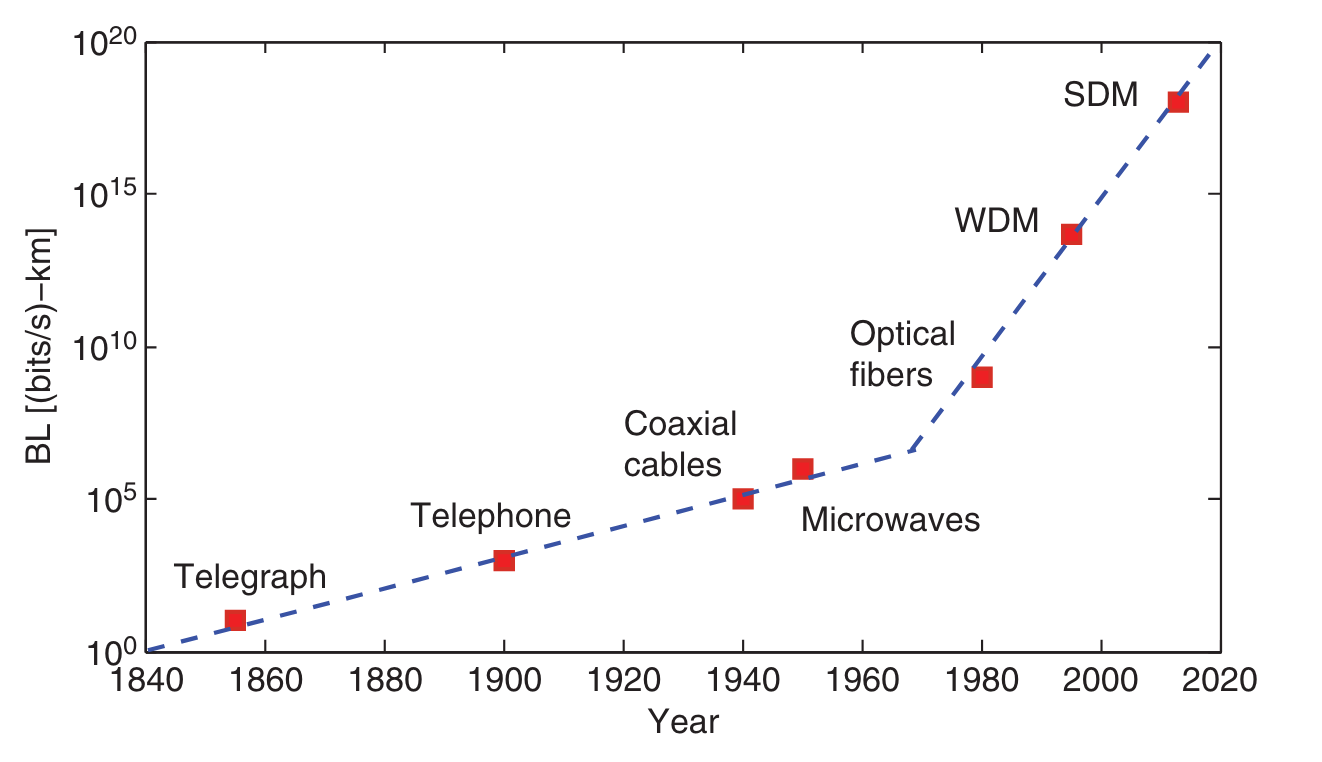
\includegraphics[width=0.45\textwidth]{images/ExpGrowthOfBL.png}
    \caption{Exponential growth of $BL$. 
    Reproduced from \cite{agrawal_fiber-optic_2022}.}
\end{figure}
According to the engineering community, 
there have been six generations of fiber-optic 
communication technology. 
Among them, 
three discoveries were key. 
\par
The first was that 
low-loss fiber is physically possible. 
Dispite the long-standing agreement that 
light is an excellent carrier for information, 
the absence of low-loss waveguide for light 
and coherent light sources 
prevented the actual implementation of 
optical communication. 
In 1970 it was realized 
\cite{kapron_radiation_1970} 
that loss in fiber can be suppressed to 
below 20dB/km around 1 $\mu$m wavelength. 
This discovery and the invention of lasers 
made possible the first implementation 
of fiber-optic communication. 
The major drawbacks were 
wide spectrum of lasers and 
large dispersion in fibers. 
\par
The second was that 
dispersion spectrum in fibers 
can be shifted so that 
the zero-dispersion wavelength 
matched that which was employed 
in communication (typically 1.55 $\mu$m). 
Dispersion-shifted single-mode fibers 
allowed the transmission of data 
at 4 Gbps across 100 km. 
\cite{gnauck_4-gbits_1985}
\par
The third was that signals could be amplified 
with optical techniques instead of digital ones, 
and that channels can be multiplexed by 
division of frequency (that is, WDM). 
This discovery coincided with the 
``internet boom'' around 2000. 
Thanks to this innovation, transmission across over 10000 km 
at 10 Gbps was realized. 
\par
It is worth noting that 
up to this time, most techniques have 
centered around linear optics. 
However, around the same time as 
amplified WDM systems were developed, 
nonlinear effects were also being 
exploited to aid communication. 
For example, in 1993, optical phase conjugation, 
an intrisically nonlinear effect, 
was used to compensate dispersion effects. 
\cite{watanabe_compensation_1993} 
Solitons 
\cite{mollenauer_solitons_2006}
, the stable solutions to the 
nonlinear wave equation, were also used to 
achieve ultra-long haul (9000 km) transmission 
at 20 Gbps in single-mode fibers. 
\cite{morita_20-gbs_1996} 
This was soon improved
\cite{mollenauer_experimental_2003}
to 
1Tbps at 18,000 km via WDM. 
This distance is already half of earth's circumference.
\par
Indeed, techniques after WDM 
have all suffered from nonlinear penalties, 
and nonlinear techniques that help 
circumvent such penalties 
have been widely deployed. 
\par
Today's most popular format is the so-called 
fifth generation communication, which is 
the improved version of WDM 
which involves larger bandwidth achieved by 
better fiber fabrication technologies and 
more bit rate enabled by coherent detection. 
\par
\begin{figure}
    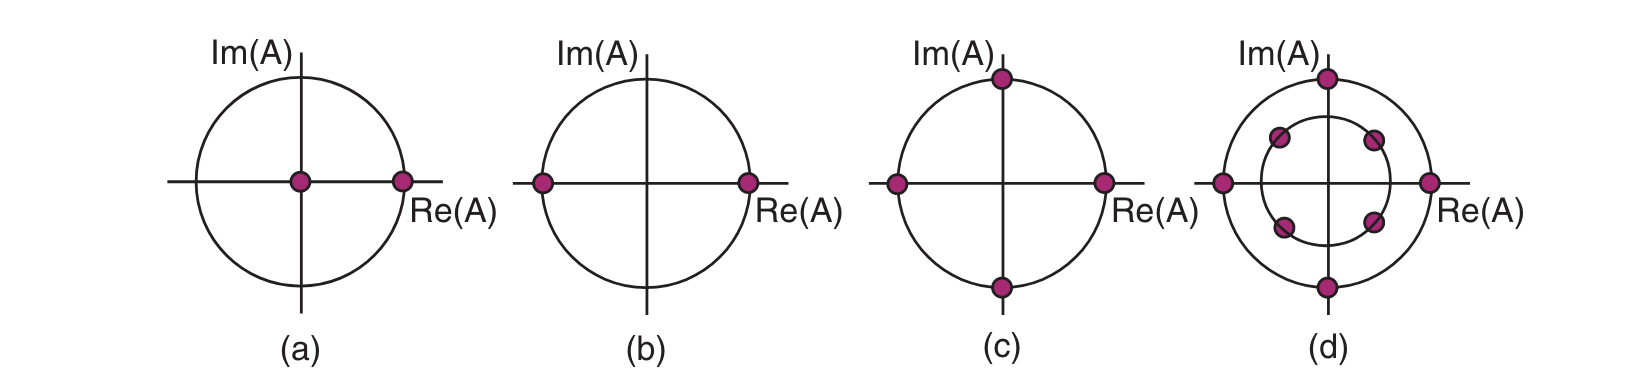
\includegraphics[width=0.45\textwidth]{images/CoherentDetection.png}
    \caption{Examples of coherent detection. 
    More precise knowledge about the phase 
    enables denser encoding. 
    Reproduced from \cite{agrawal_fiber-optic_2022}. }
\end{figure}
Around the 2010s, single-channel capacity 
approached the Shannon limit. 
\cite{ellis_approaching_2010,essiambre_capacity_2010}
This strengthened the belief that 
further improvement in fiber-optic systems 
could only be extracted 
by exploiting novel multiplexing schemes. 
Today's state-of-the-art 
fiber-optics systems are indeed advanced multiplexing 
systems, for example space-division systems 
\cite{saitoh_multicore_2016}
that achieve 1000 Tbps at 1000 km, and 
Petabit-per-second systems that combine 
WDM and SDM \cite{jorgensen_petabit-per-second_2022}. 
\par
As will be articulated in the following sections, 
although nonlinearity can obstruct communication 
in many settings, techniques exploiting nonlinearity 
turn out to be very helpful. 
\section{Nonlinear Phenomena in Optical Fibers}
Nonlinear material response to 
electromagnetic drive creates a host of 
phenomena that affects communication. 
Nonlinearity becomes 
appreciable under large drive intensity, 
which is exactly the case with optical fibers 
because its tiny core area. 
Besides, phase-modulation effects typically 
lead to a phase change proportional to the 
distance of propagation 
\begin{equation}
    \label{eqn:NonlinearPhaseShift}
    \phi_{\text{NL}}
    =
    \Delta k_{\text{NL}} z
\end{equation}
which is amplified by large $z$ 
in practical systems. 
\par
In single-mode fibers the dominant nonlinear effect 
is \textbf{self-phase modulation} (SPM), 
while in WDM and SDM systems more nonlinear effects, 
including \textbf{cross-phase modulation} (XPM) and 
\textbf{four-wave mixing} (FWM) set in. 
\par
In this section we 
review the basics of nonlinear response, 
examine the dominant nonlinear effects 
in fiber optics, 
articulate past achievement in 
utilizing nonlinearity for communication, 
and comment on the relation between 
the physical aspects of nonlinear optics and 
the engineering challenges of fiber communication. 
\subsection{Self Phase Modulation}
In fiber cores, centrosymmetry of silica glass 
leads to a vanishing $\chi^{(2)}$. Therefore, 
the dominant nonlinear optical effects is fibers 
are mostly $\chi^{(3)}$ effects. 
In the 3rd order polarization there is a term 
\[
    \vb*{P}^{(3)}
    =
    \varepsilon_0
    \chi^{(3)}
    \vb*{E}^{3}
    =
    (\varepsilon_0 \chi^{(3)}/8)
    (3 \tilde{E}_{+}\tilde{E}_{-}+c.c.)
\]
which has the same frequency as $\tilde{E}$. 
This leads to a modified refractive index 
which is dependent on the optical power 
\[
    \Delta \chi^{(1)}
    =
    \frac{3}{4}\chi^{(3)}\abs{E} ^{2}.
\]
\par
In fact, this can happen 
not only within one channel, 
but also between channels. 
\par
Because $k=\frac{n(\omega)\omega}{c}$, 
insert Eqn. \ref{eqn:NonlinearPhaseShift} and 
$n=\sqrt{1+\chi^{(1)}}$ we see that 
SPM will lead to a phase shift proportional to $z$. 
\par
Broadening the pulse so that 
peak intensity lowers is a solution to this problem. 
Efforts in managing logal dispersion 
have met engineering challenges in optimizing the 
arrangement of local dispersion. 
(See Fig.~\ref{fig:ThreeDMaps} for three different arrangements that are expected to yield the same result 
but turn out not to.)
\begin{figure}
    \label{fig:ThreeDMaps}
    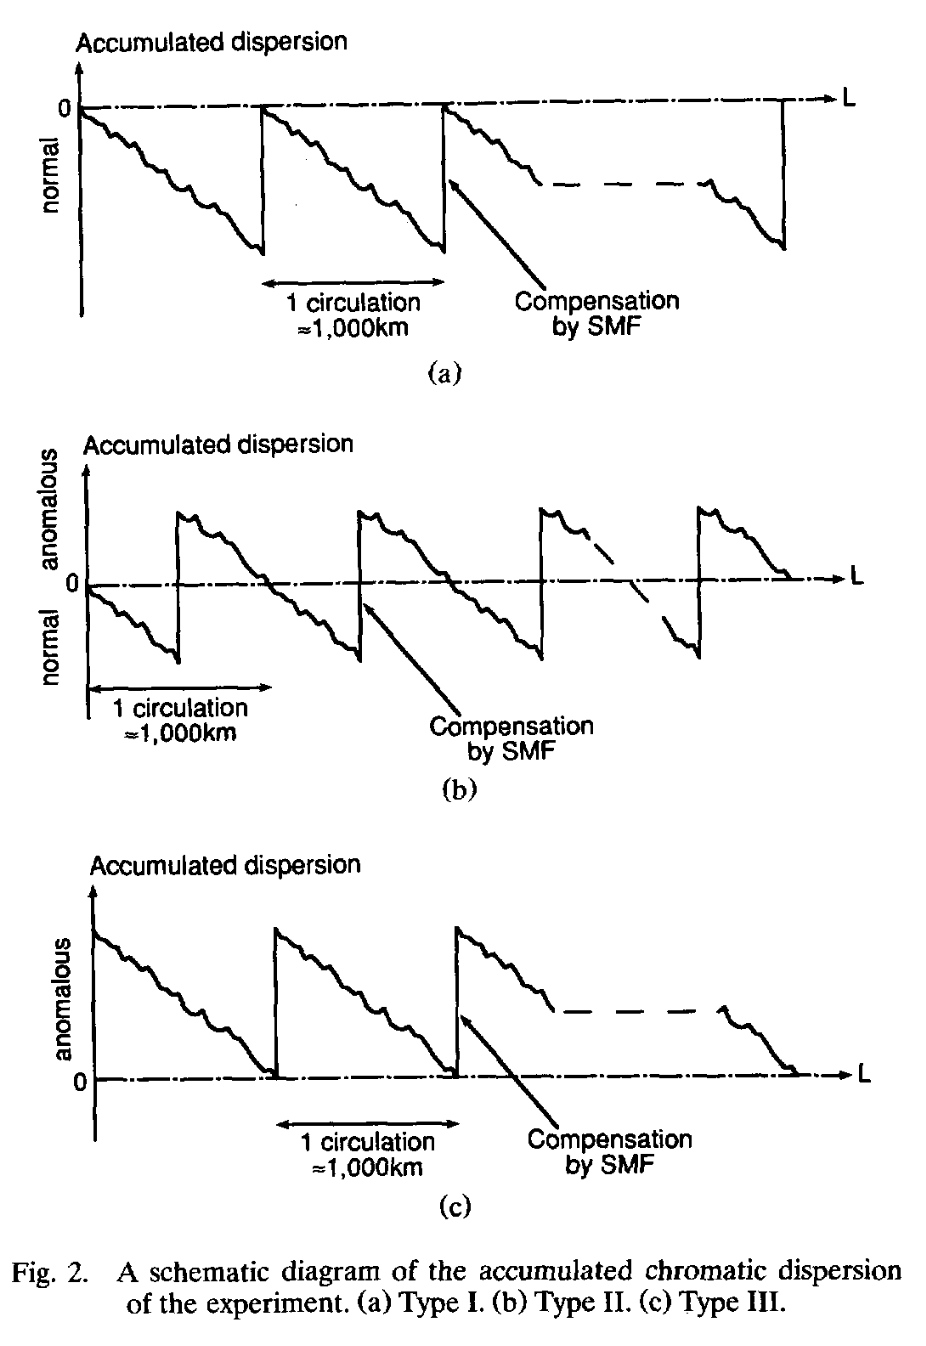
\includegraphics[width=0.45\textwidth]{images/ThreeTypesOfDM.png}
    \caption{Three different types of 
    dispersion arrangement. 
    The ``anomalous'' dispersion region corresponds to negative $k_2$ values. 
    Reproduced from \cite{taga_performance_1994}.}
\end{figure}
\subsection{Temporal Soliton}
Temporal soliton results from the combined effort of 
GVD and SPM. 
By taking the Fourier transform on the 
envelope propagation equation
\[
    \pdv{\mathcal{E}}{z}
    -
    \mathrm{i}\mathcal{E} \delta k
    =0,
\]
we obtain 
\begin{equation}
    \label{eqn:DispersionEquation}
    \pdv{\mathcal{E}}{z}
    +
    k_1
    \pdv{\mathcal{E}}{t}
    -
    \mathrm{i}k_2
    \pdv[2]{\mathcal{E}}{t}
    +
    k_3
    \pdv[3]{\mathcal{E}}{t}
    -
    \mathrm{i}\Delta k_{\text{NL}}\mathcal{E}
    =0.
\end{equation}
This is a more careful treatment of 
dispersion in optical fibers than 
the rough estimatino given in Eqn. \ref{eqn:CriterionGVD}. 
Ignoring $k_3$ and 
inserting 
\[
    \Delta k_{\text{NL}}=
    \frac{n_2^{(I)}\omega_0}{c}, 
    \quad 
    \tau \equiv t-\frac{z}{c}
\]
we obtain the \textbf{nonlinear Schrodinger equation} (NLSE), 
\begin{equation}
    \pdv{\mathcal{E}}{z}
    +
    \mathrm{i}k_2
    \pdv[2]{\mathcal{E}}{t}
    =
    \mathrm{i} \gamma \abs{\mathcal{E}} ^{2} \mathcal{E}.
\end{equation}
This is the equation that governs 
the formation of temporal solitons. 
\subsubsection{Soliton Formation}
In Eqn.~\ref{eqn:DispersionEquation} the term 
$\pdv[2]{\mathcal{E}}{\tau}$ is typically negative 
at the pulse peak. Therefore 
the GVD term and nonlinear term will cancel each other 
only if $k_2$ and $n_2^{(I)}$ has opposite signs. 
When their effects cancel each other exactly, 
the pulse will neither broaden with dispersion 
nor broaden because of nonlinearity. 
\par
This balance between GVD and SPM gives the 
\textbf{soliton} solution to the NLSE, 
which is a family of surprisingly stable pulse. 
The lowest-order soliton is a sech-profile packet. 
\cite{mollenauer_solitons_2006}
\par
In this light the dicision as for 
which among the three dispersion arrangements 
in Fig.~\ref{fig:ThreeDMaps} becomes trivial. 
Because the $k_2<0$ region effectively 
compensates for SPM, the nonlinear penalty 
will be alleviated even though there is no soliton, 
because the compensation is not yet enough. 
Therefore the optimal arrangement should be that which 
maximizes the propagation length in the anomalous 
dispersion region, which is type (c) in the figure. 
This aligns with the result 
obtained in \cite{taga_performance_1994}.
\subsubsection{Soliton Stability}
Solitons are stable. Because this is a well-defined 
differential equation problem, mathematicians 
\cite{tao_why_2008,newell_solitons_1987} 
have developed relevant theories and made predictions. 
\par
There are also physical perspectives. 
One is that just as fibers are spatial waveguides 
that trap light inside, 
the SPM effect essentially constitutes a 
temporal waveguide that trappes the pulse 
in its most intense regions. 
\begin{figure}[h]
    \label{fig:TwoKindsOfWaveguide}
    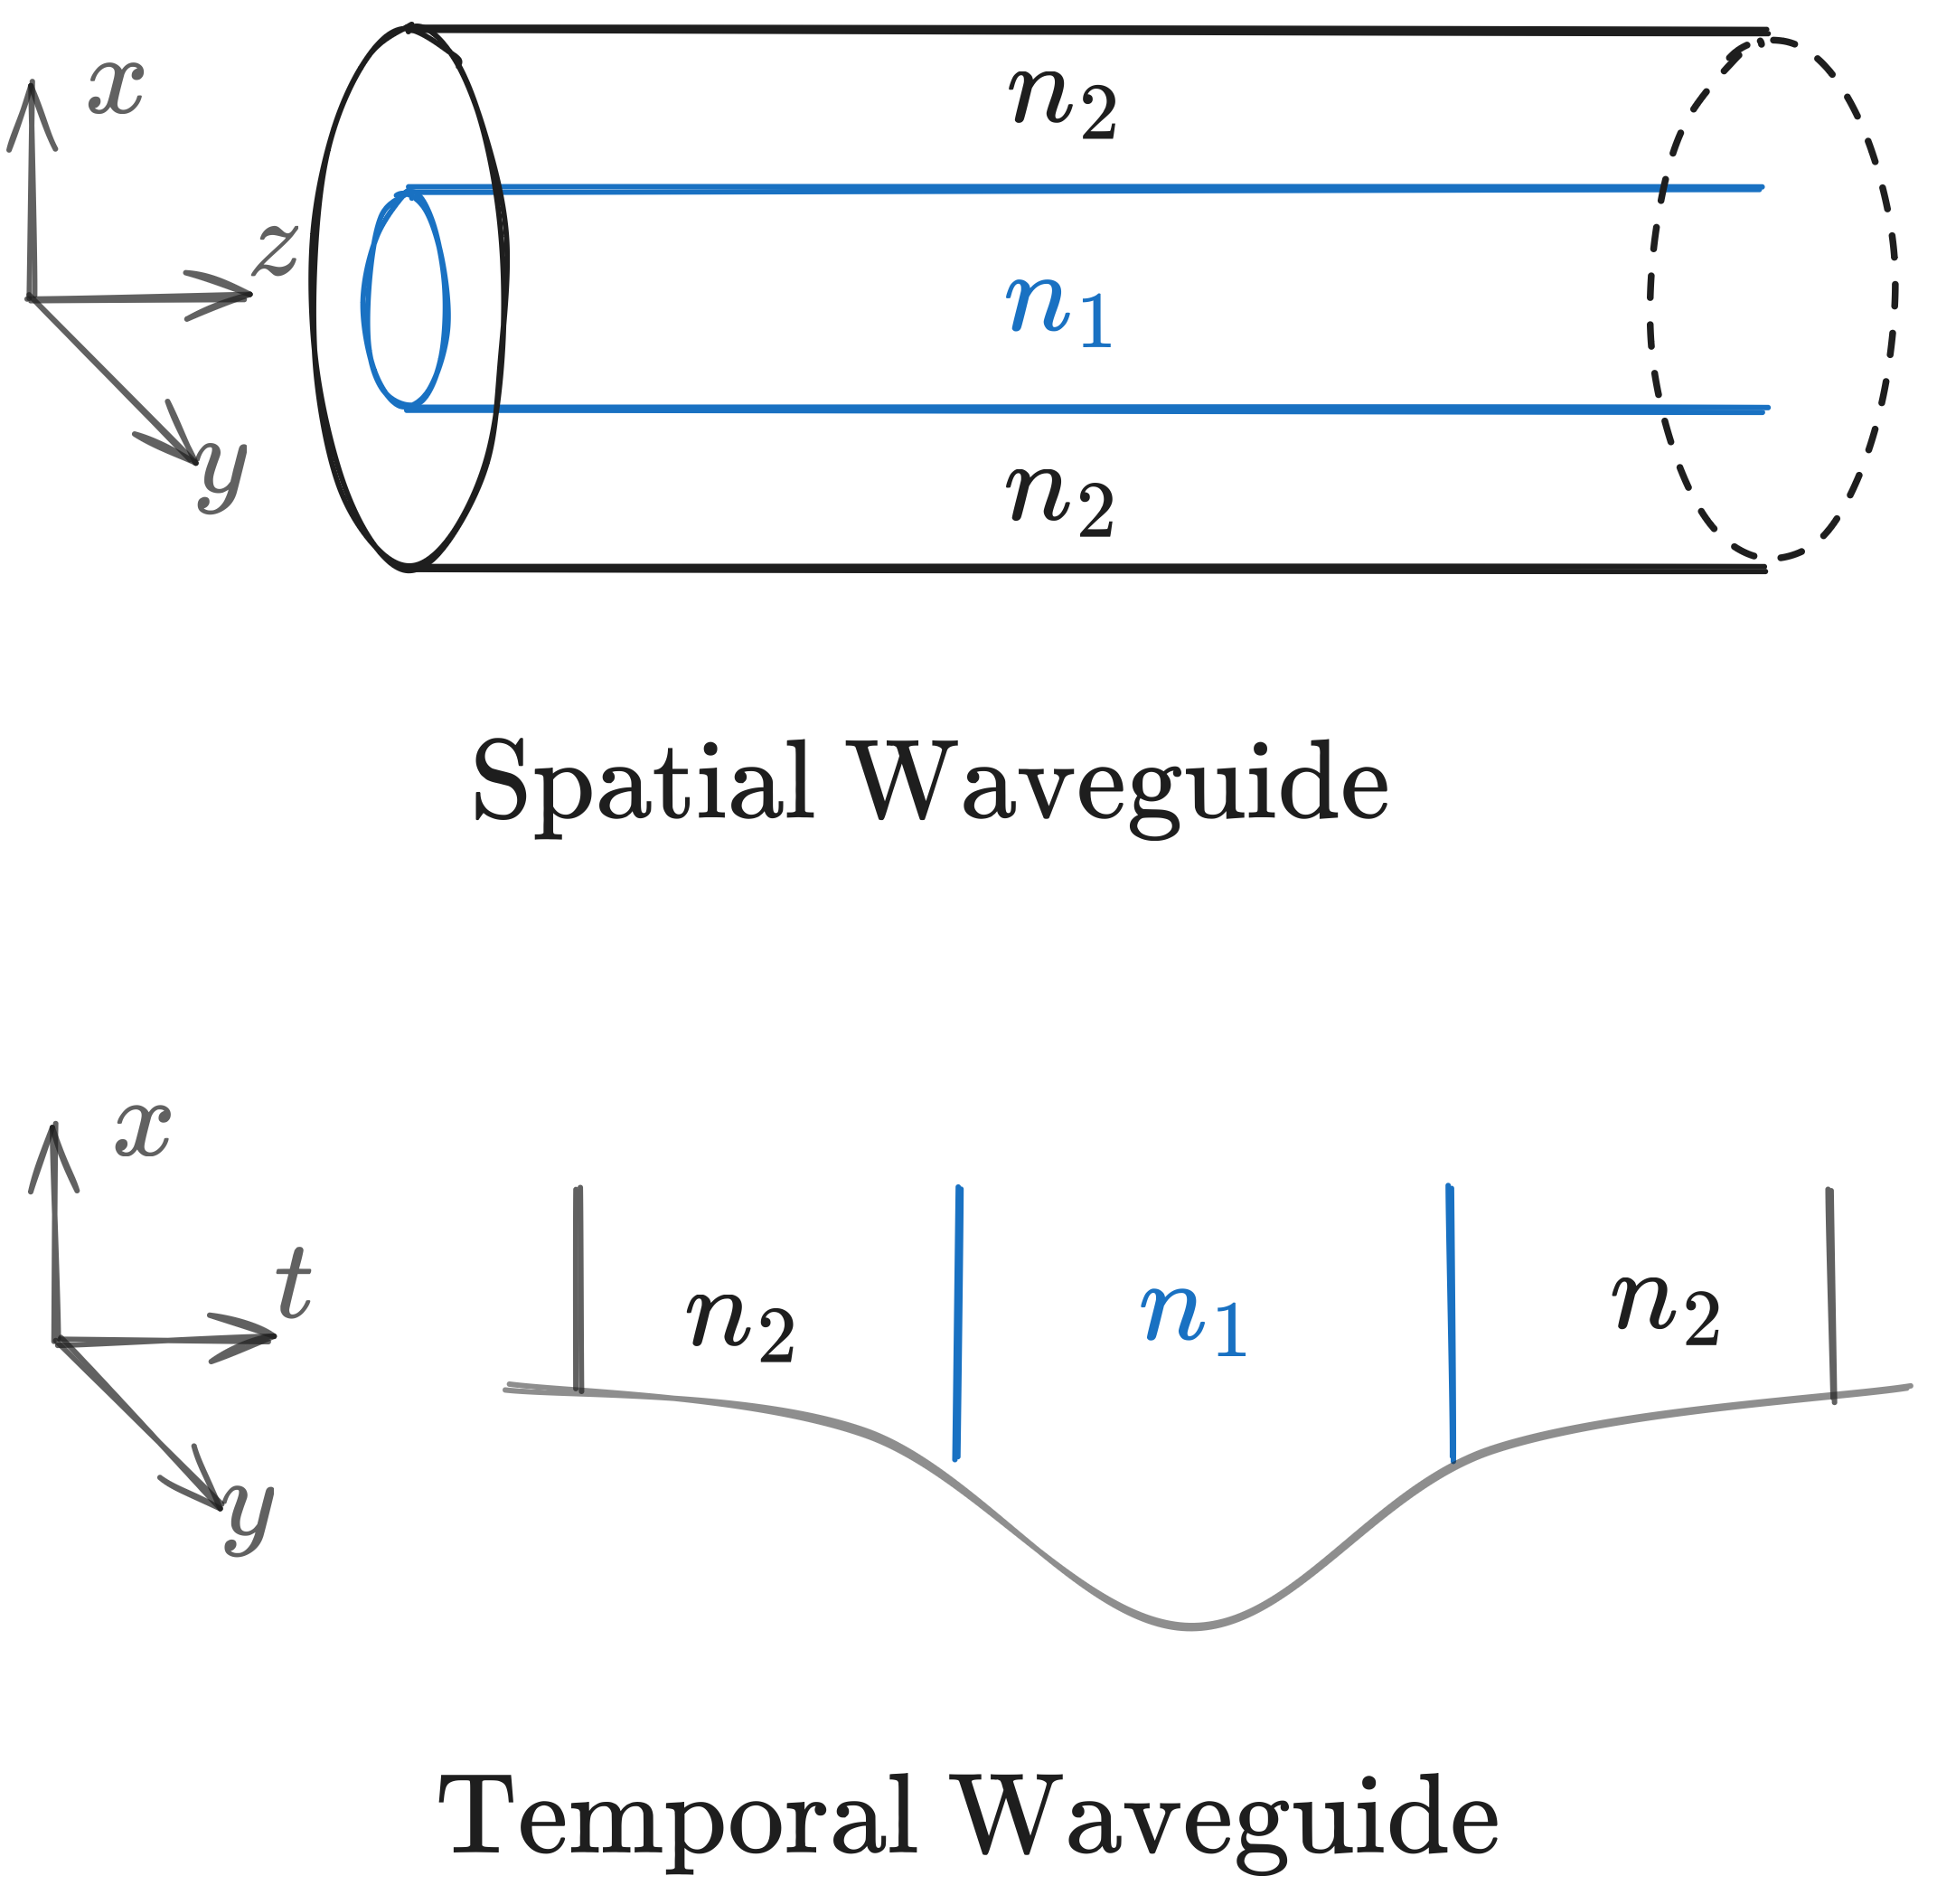
\includegraphics[width=0.45\textwidth]{images/TwoKindsOfWaveguide.png}
    \caption{Diagram that shows two kinds of waveguides. 
    Here $n_1>n_2$ in both waveguides. }
\end{figure}
\par
This waveguide moves at the speed that is equal to 
that of pulse propagation, 
thus maintaining its profile throughout the fiber. 
Indeed, the notion that solitons are 
``self-trapped'' pulses matches the NLSE. 
In the NLSE the potential energy term 
is 
\[
    V=-\gamma \abs{\mathcal{E}}^{2} , 
\]
and a positive SPM coefficient $\gamma$ indicates that 
the potential is not a barrier but a well 
(see Fig.~\ref{fig:TwoKindsOfWaveguide} for an intuition). 
However, while the Schrodinger equation 
describes evolution in time, 
the NLSE describes evolution in \textit{space}. 
Directly comparing the NLSE and the Schrodinger equation 
will make this clear. 
Add to this the fact that the co-moving frame time 
$\tau$ instead of $t$ appears in the equation, 
its exact meaning becomes opaque. 
Upon examining the behavior of the NLSE 
with only the dispersive term or 
only the nonlinear term, we can see that 
\cite{mollenauer_solitons_2006}
both cause spreading of the ``wavepacket'' 
in the spatial coordinate. 
We may conclude that despite the name NLSE, 
intuition provided by the quantum mechanics analogy concerning this equation is limited.
\par
One profound evidence for soliton stability is 
the existence of \textbf{dispersion-managed solitons}. 
Even though a negative $k_2 n_2$ is required for 
soliton formation, 
experiments 
\cite{morita_20-gbs_1996}
have shown that solitons can survive 
regions where $n_2 k_2>0$ as long as the 
\textit{path-averaged} value of $k_2 n_2$ is appropriate. 
\par
Another evidence for soliton stability is that 
when non-soliton pulses are incident into 
fibers, the pulse shape approaches the soliton shape 
as it propagates. This can be viewed as 
the effect of a waveguide on pulses where 
only the supported modes survive propagation, and 
here the supported modes of the temporal waveguide 
is a series of soliton solutions. 
\begin{figure}
    \centering
    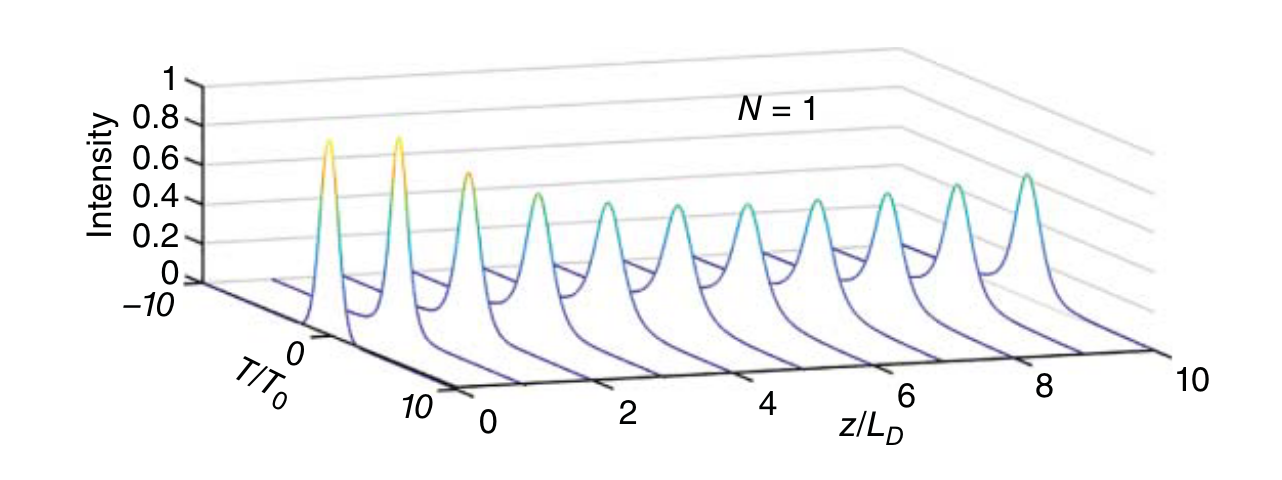
\includegraphics[width=0.45\textwidth]{images/Imperfect_Pulse.png}
    \caption{Numerical result of a Gaussian profile 
    incident into nonliner fiber. 
    As $z$ increases the shape approaches 
    that of a fundamental soliton. 
    Reproduced from \cite{agrawal_fiber-optic_2022}.}
\end{figure}
\subsubsection{Applications of Soliton in Communication}
Solitons were initially predicted 
\cite{hasegawa_transmission_1973}
and experimentally demonstrated in a commercial lab. 
\cite{mollenauer_experimental_1980} 
Because of their stable nature, solitons 
have since been candidates for fiber-optic communication, 
especially ultra-long haul transmission. 
Although GVD is balanced out by SPM in solitons, 
fiber loss, 
other nonlinear effects, and soliton collisions, 
can undermine soliton fiber systems' performance. 
\par
The most significant breakthrough was the 
implementation of dispersion-managed solitons 
\cite{morita_20-gbs_1996}. 
Because in the presence of fiber loss 
maintaining the pulse shape of solitons is impossible, 
researchers gave up maintaining this shape and 
decided to construct the fiber system so that 
pulse shapes of solitons evolved periodically. 
This was achieved by using techniques similar to 
that of dispersion management (DM), where 
$k_2$ were engineered to alternate between positve and 
negative values as the signal propagates, resulting 
in the receiver a net dispersion of zero. 
It turned out that even after this periodic evolution 
the pulse shapes could be recovered quite accurately 
without additional digital effort. Soliton signals 
were transmitted across 9,000 km 
with DM as the only compensation scheme. 
\par
Although solitons are not spectrally the most efficient 
pulses because they are sharp pulses that occupy 
a broad bandwidth, 
they can still be integrated into WDM systems. 
Unlike linear signals that suffer from 
the usual nonlinear penalties, 
solitons have their own unique dynamics and 
noise model, for example the 
timing jitter caused by soliton collision. 
In order to compensate for 
such effects, techniques specifically designed for 
soliton systems were invented. 
For example, Periodic-group delay method 
compensates for a large proportion of timing jitter, 
resulting in a 18,000-km soliton system 
operating 109 channels with WDM at a total 
bit rate of 1 Tbps. 
This distance is more than enough for 
the global internet, which again shows the 
benefit from soliton stability. 
\subsection{Four-wave Mixing}
In WDM systems, channels that occupy 
nearby bands can interact via four-wave mixing (FWM). 
From a quantum optical point of view this is 
the annihilation of two photons 
and the creation of two other photons 
with energy conserved. 
This process exchanges energy between channels, 
thus inducing severe cross-talk noise 
that harms communication severely, 
because this is dissipative noise 
and can not be compensated for. 
\par
From a nonlinear optical point of view 
FWM can be described by 
\begin{equation}
    \label{eqn:CoupledWaveEquationForFWM}
    \dv[]{A_{l}}{z}
    =
    - \frac{\alpha}{2}
    A_{l}
    +
    d \chi^{(3)}_{\ell ijk}
    A_{i}A_{j}A^{*}_{k}
    \exp(-\mathrm{i} \Delta k z)
\end{equation}
with 
\[
    \alpha =\text{ fiber loss and }
    \Delta k
    \equiv 
    k_{l}+k_{k}-k_{i}-k_{j}.
\]
For nearby channels $l,i,j,k$ with equal 
frequency spacings, this effect is severe 
provided that $\Delta k$ is small. 
This is the \textbf{phase matching} condition 
for FWM. 
\par
In this light, the cure to FWM 
can be DM: introducing a phase shift so that 
even nearby channels can not achieve phase matching 
during propagation, and engineer the system so that 
net dispersion is zero at the receiver. 
\subsection{Cross Phase Modulation}
Cross phase modulation (XPM) is the inter-channel counterpart 
of SPM. For example, in a WDM system, 
between three equally spaced channels at frequencies 
\[
    \omega_1<\omega_2<\omega_3
\]
a polarization term 
\[
    \tilde{P}^{(3)}_{i}(\omega_2)
    =
    \varepsilon_0
    \chi^{(3)}_{ijk\ell}
    (\omega_2;\omega_1,\omega_3, -\omega_2)
    \tilde{E}_{j}(\omega_1)
    \tilde{E}_{k}(\omega_3)
    \tilde{E}^{*}_{\ell}(-\omega_2)
\]
is possible. Therefore the refractive index of channel $\omega_2$ 
can be modulated by 
\[
    \Delta \chi^{(1)}
    =
    \frac{3}{4}
    \chi^{(3)}_{ijk\ell}
    \abs{E_{j}E_{k}}. 
\]
Similar to compensation against SPM, XPM can be alleviated via DM. 
\subsection{Optical Phase Conjugation}
Optical phase conjugation (OPC) is an efficient technique 
to compensate for \textit{single-channel} phase shift noise. 
Recalling Eqn.~\ref{eqn:NonlinearPhaseShift}, 
if the phase of signal is reversed at the middle point $z /2$ 
during propagation, the total acquired phase shift would be 
\[
    \Delta k_{\text{NL}}(z+(-z))/2=0,
\]
which is the desired result. 
\par
OPC can be achieved either through FWM or 
DFG; in practice it is often implemented via PPLN waveguides 
in a combinatino of SHG and DFG processes \cite{jansen_long-haul_2006}. 
\par
This method is powerful because 
it does not rely on any specific phase shift mechanism; 
as long as phase shift is proportional to propagation length, 
OPC can alleviate the noise significantly. 
For example, it can account for both SPM and GVD. 
Another advantage of OPC is frequency independence. 
In WDM systems OPC can be employed to simultaneously account for 
phase shift error in multiple channels. 
\cite{jansen_long-haul_2006}
\par
However, OPC can \textit{not} account for inter-channel noise, 
such as XPM. This is because 
$\Delta \phi_{\text{Interchannel}}$ is a function of DM arrangement and 
frequency difference between channels, among other parameters, 
which breaks down the proportional relation of $\Delta \phi$ with $z$. 
\par
OPC can be combined with DM to account for FWM. For example, 
before executing the usual OPC scheme one may 
run the signal through some pre-compensation fiber 
and after OPC the signal can be subject to a post-compensation fiber 
so that net accumulated dispersion at receiver is zero. 
\begin{figure}[h]
    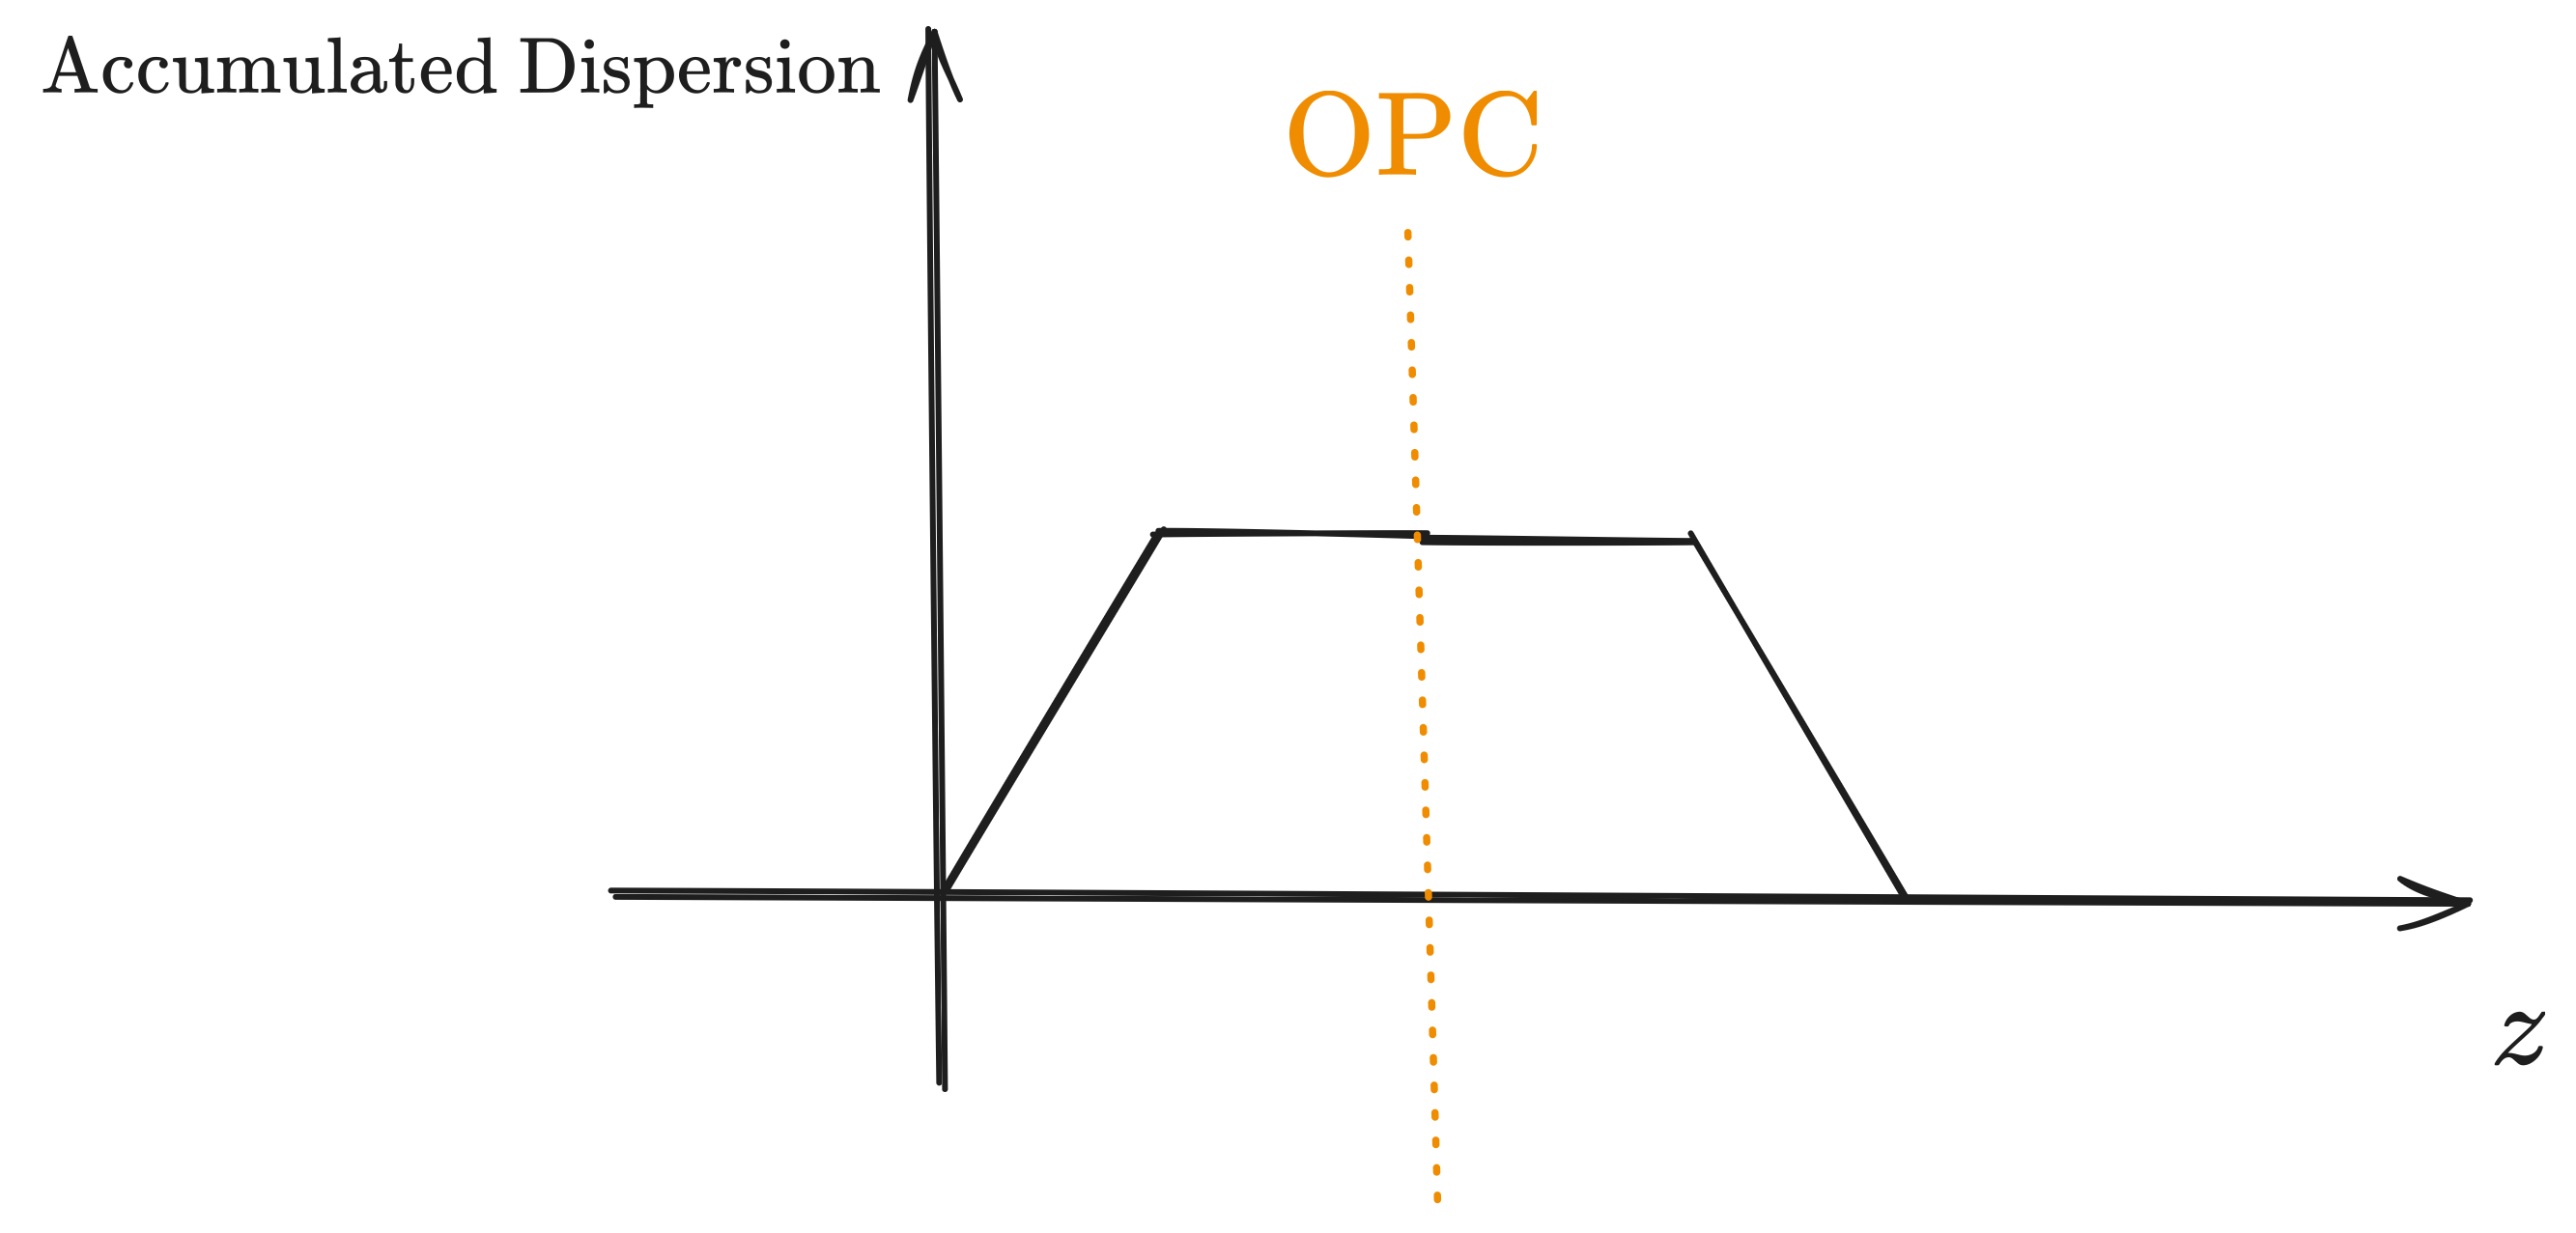
\includegraphics[width=0.45\textwidth]{images/OPC_And_DM.png}
    \caption{Accumulated dispersion as a function propagation length.}
\end{figure}
\section{Discussion and Outlook}
To sum up, the various noise and compensation schemes can be summarized as 
shown in the below table. The table elements Y/N indicates wheter 
the corresponding compensation scheme is able to cancel the noise source. 
\begin{table}[h]
    \begin{tabular}{ccc}
    \toprule
    Noise
    &
    OPC+DM
    &
    Soliton+DM\\
    \midrule
    FWM
    &
    Y
    &
    Y
    \\
    SPM
    &
    Y
    &
    Y
    \\
    GVD & Y & Y \\
    XPM & N & Y \\
    \bottomrule
    \end{tabular}
    \caption{Summary of noise sources and compensation schemes. 
    Note that XPM is overshadowed by collision-induced timing jitter 
    in soliton systems. }
\end{table}
Nonlinear effects constitute the primary obstacle in 
improving single-channel capacity as well as multiplexing efficiency. 
However, by exploiting nonlinear effects we have also obtained 
a rich collection of tools that improve fiber-optic communication systems. 
While soliton systems are not the focus of current research 
due to their low spectral efficiency and stringent modulation requirements, 
their stability have enabled pioneering work on ultra-long haul 
fiber optic transmission. More importantly, 
relevant scientific progress has falsified the misconception that 
nonlinear effects are merely incomprehensible noise that 
can only be circumvented through engineering and optimization. 
Phenomena previously deemed as engineering challenges 
have turned out to be physically understandable. 
Tapping into the rich physics of nonlinear optics has paid off well 
for the fiber-optic communication community. 
\subsection{Space Division Multiplexing}
The current focus of fiber-optic communication is multiplexing techniques. 
Among the various multiplexing schemes now under development the 
most promising one is space division multiplexing (SDM). 
\par
As the name suggests, SDM is multiplexing channels by 
separating them spatially while integrating them into the same 
fiber. This requires the fiber to have either multiple modes 
or multiple cores. 
Non-fundamental transverse modes of fiber are more prone to noise, therefore 
the better choice would be to use multi-core fiber for SDM. 
\par
Quite surprisingly, multi-mode effects in SDM can compensate for SPM 
as well as XPM. Running multiple cores at the same time not only 
does not induce more nonlinear noise but also turns out to suppress it. 
This can be read off the following equation
\[
    \Delta k_{i}
    =
    \sum_{\ell,m,n}
    \chi^{(3)}_{i,\ell,m,n}
    E_{\ell}E_{m}E^{*}_{n}
    +
    \sum_{p}q_{i,p}E_{p}
\]
with $q_{i,p}$ the linear coupling constant between 
different fiber cores, and $\chi^{(3)}_{i,\ell,m,n}$ the 
susceptibility. \cite{mumtaz_reduction_2012}
The refractive index difference between fiber core and cladding 
introduces a phase shift into in-phase signals when they couple, 
thus producing a negative sign in $q_{i,p}$ (see the diagram for 
an intuition). 
Therefore, in SDM systems both XPM and SPM are alleviated 
by the inter-core coupling. 
In this light, manufacturers have tested multi-core fibers 
that are deliberately made so that coupling between cores is strong. 
Today's most advanced SDM systems can achieve up to 1000 Tbps 
at 1000 km. \cite{saitoh_multicore_2016}
\begin{figure}[h]
    \centering
    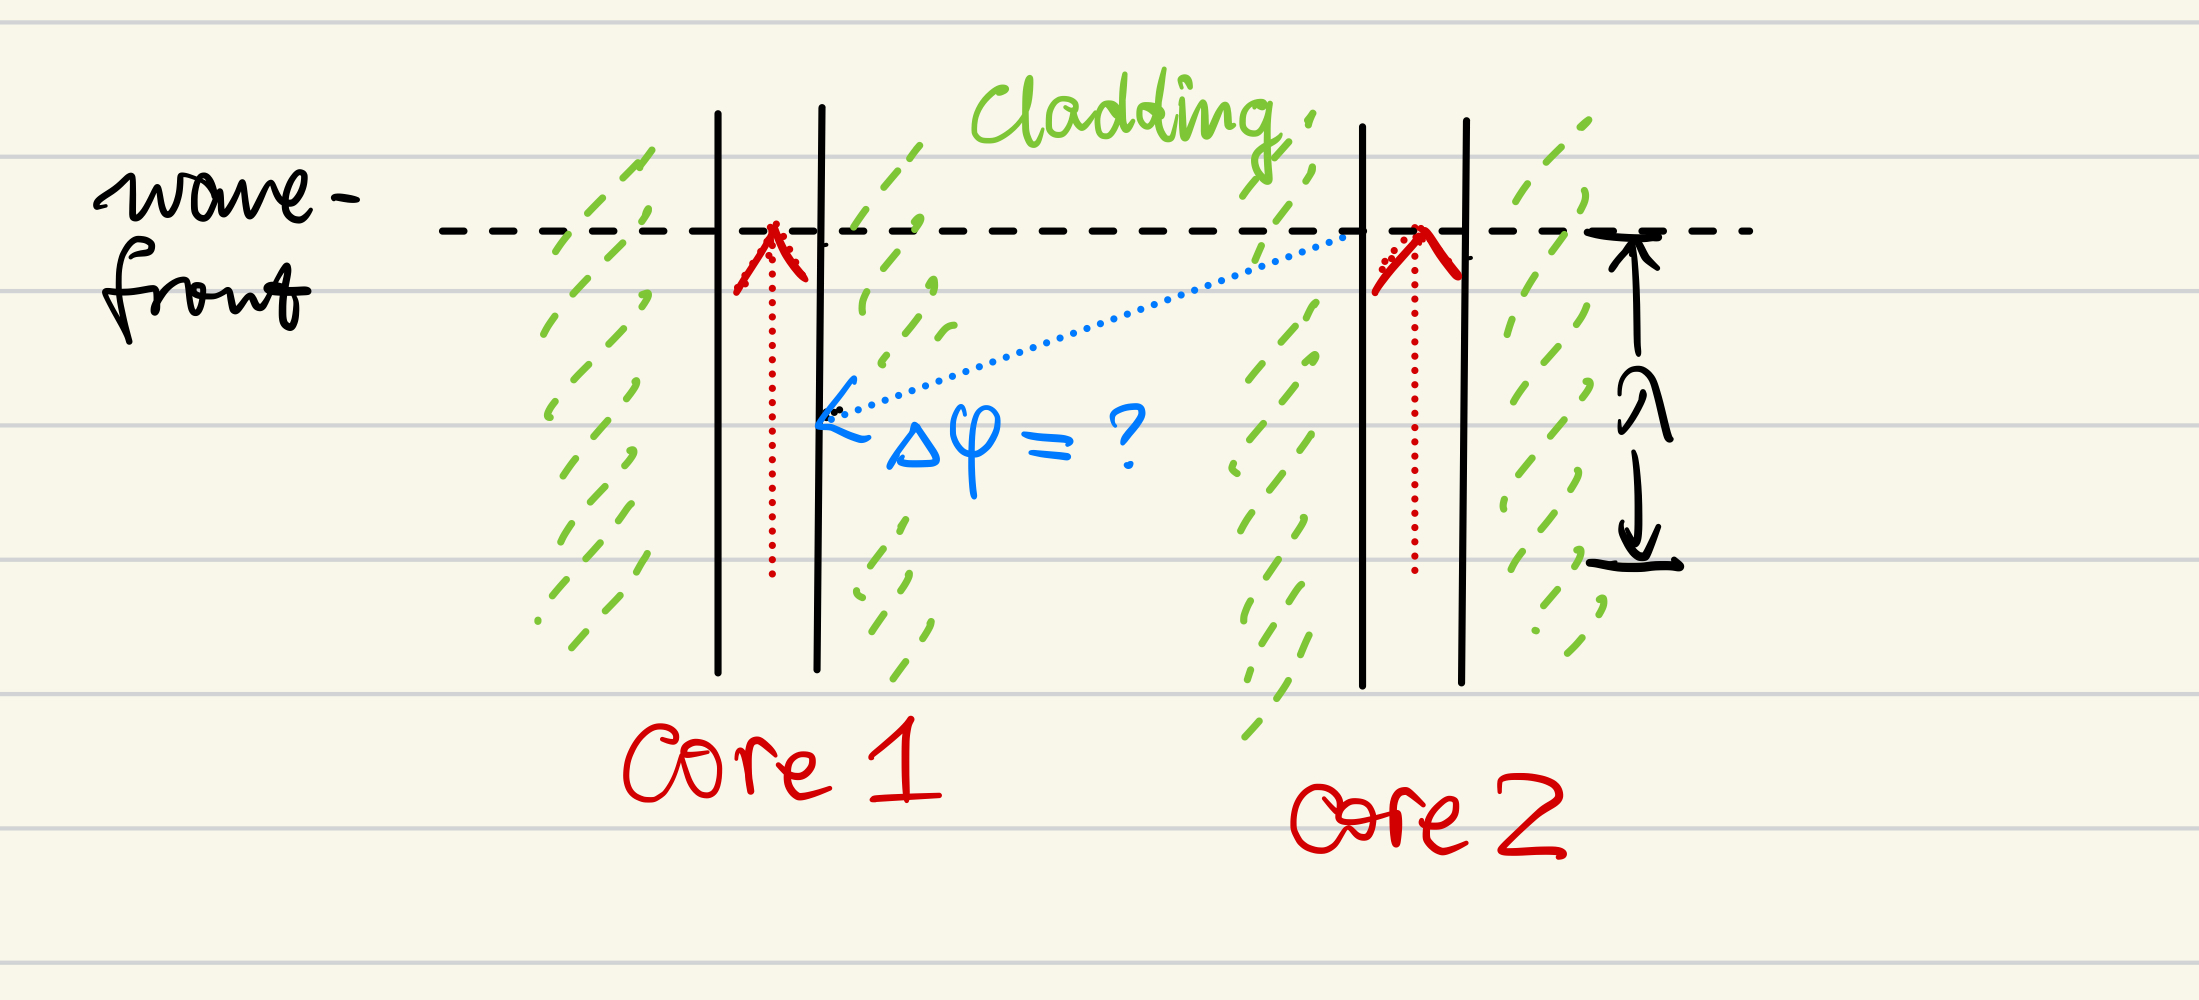
\includegraphics[width=0.45\textwidth]{images/Intercore_Coupling.jpeg}
    \caption{Phase difference between 
    different cores' signals lead to various effects 
    because the transverse profile is also delayed by this phase. 
    The blue text showing $\Delta \phi=?$ indicates that 
    specifics depend on the physical apparatus. Here the delay 
    is half-wavelength phase shift. }
\end{figure}
\subsection{Nonlinear Fourier Transform}
The nonlinear Fourier Transform (NFT), also known as the 
\textbf{backward scattering} technique, 
is the mathematical formalism for determining the 
eigenmodes of a nonlinear propagation channel. 
The motivation behind using this technique for communication is that 
by encoding information in the eigenvalues 
\cite{hasegawa_eigenvalue_1993}, more than 1 bit of information 
can be sent within one pulse time, and 
this pulse will not be subject to any nonlinear noise. 
The motivation is shown in the diagram below.  
\begin{figure}
    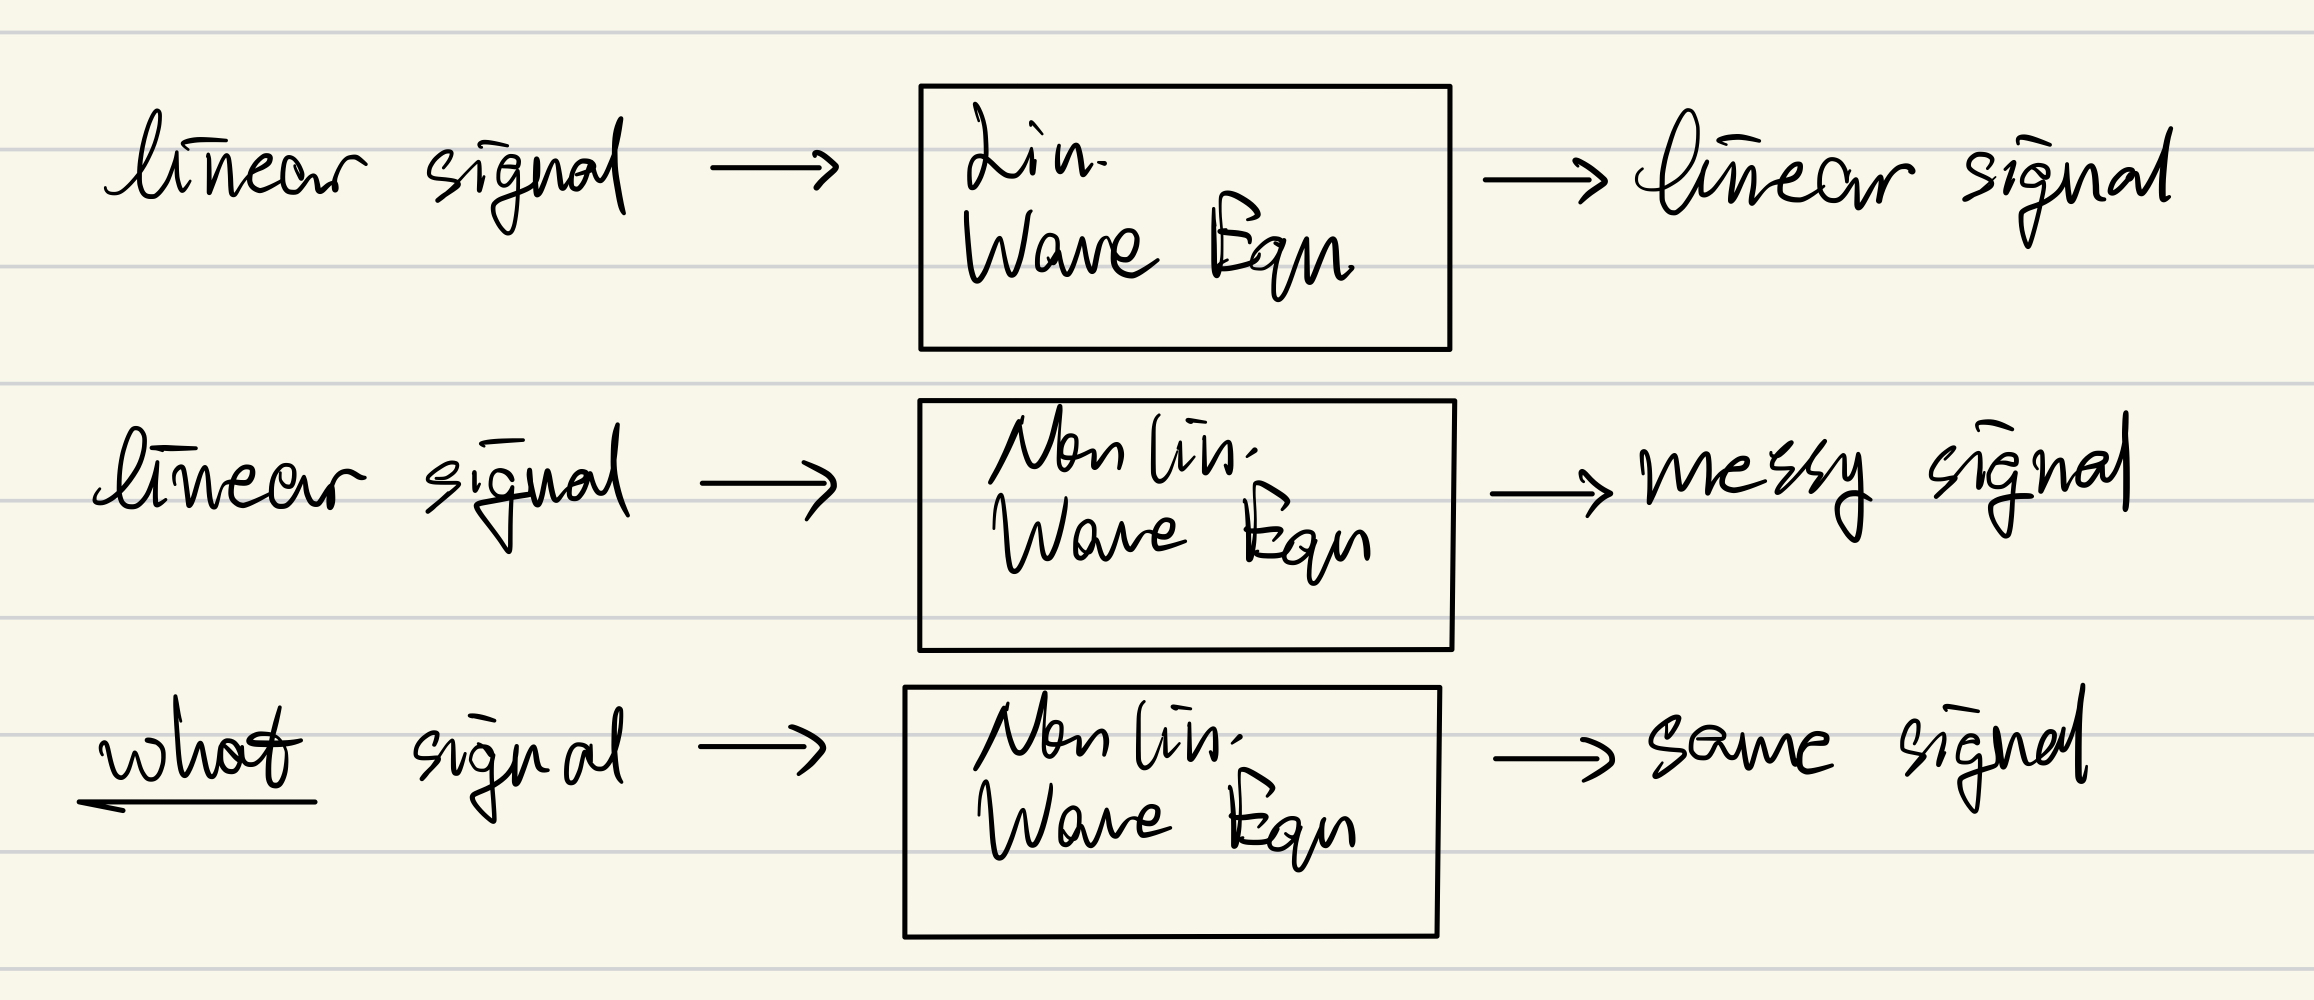
\includegraphics[width=0.45\textwidth]{images/IdeaOfNFT.jpeg}
    \caption{A simple diagram that motivates the NFT. 
    We already know the properties of the first two lines, 
    and are exploring the possibility of using the third line 
    for communication.}
\end{figure}
This technique is still in its infancy, 
and similar to the soliton technology with 
wasn't competitive until challenges particular to that technology 
were addressed, the NFT is a promising technique that 
has passed numerical tests \cite{le_high_2018,prilepsky_nonlinear_2014} but awaits further development. 
\par
\bibliographystyle{plainnat}
\bibliography{apssamp}% Produces the bibliography via BibTeX.

\end{document}
%
% ****** End of file apssamp.tex ******
